%%%%%%%%%%%%%%%%%%%%%
% turnout - Switch
% three-way turnout
% 
\documentclass{article}
\usepackage[a4paper]{geometry}
\usepackage[american]{babel}
\usepackage[utf8]{inputenc}
\usepackage{modeltrain}
\usepackage{graphicx}
\usepackage{pgffor}
\usepackage{sverb}
\usepackage{listings}
\lstset{language=TeX,mathescape=true,frame=Trbl,numbers=left}
\author{Dietrich Paulus}
\title{ModelTrain}
\date{Vers. 0.1 \\ \today}
\def\RoomLength{400}
\def\RoomWidth{250}
\def\Example#1#2#3#4{%
 \lstinputlisting[% float,%
    % firstline=#2,%
    % lastline=#3,%
    % firstnumber=#2,%
 	% frame=\frame,%
 	% index=\INDEXWORDS,%
	basicstyle=\ttfamily\small,%
	keywordstyle=\ttfamily\small,%
	commentstyle=\rm,%
	label=ex:#1,%
	caption={#4}]{#1}%
}

\parindent=0pt
\parskip=1ex

\begin{document}

\maketitle

\tableofcontents

\newpage

What is the idea behind the following package?
\begin{itemize}
  \item I want to create a track layout for a model train.
  \item I program the layout in a sequence of steps; these steps
     correspond to the steps that I would do in reality with real (model) tracks.
  \item Programming the layout should be done with \LaTeX\ and Tikz.
\end{itemize}


\section{Strategy}

The typical steps are as follows:
\begin{enumerate}
  \item We select a plane size and shape on which we want to lay the tracks.
     (We do this as a polygon in Tikz).
  \item We select a starting point for the tracks in Tikz coordinates.
  \item From the starting point on we lay tacks and connect them sequentially.
  \item We select tracks of the following types:
     \begin{enumerate}
       \item straight tracks (of varying length)
       \item curved tracks (of varying angle and radius)
       \item switches (of different types)
     \end{enumerate}
\end{enumerate}


\section{Track Names}

For Märklin, the following track names are admissible:
% \makeatletter
\foreach \i in \TrackNameList{\i, }
For curves we need to use either \texttt{LCurve} or \texttt{RCurve} to indicate the direction.

%%%%%%%%%%%%%%%%%%%%%%%%%%%
\section{First Examples}

We start with a small complete example without switches, as shown in the following:

\begin{verbwrite}{example1}
\documentclass{standalone}
\usepackage{modeltrain}
\begin{document}
\begin{tikzpicture}[scale=0.06]
  \draw (0,0) -- (100,0) -- (100,85) -- (0,85) -- cycle; %% frame

  \draw (40,05)    % start layouting tracks here
    \Straight{5106}  % start with a straight track
    \LCurve{5100}  % 6 curves
    \LCurve{5100}
    \LCurve{5100}
    \LCurve{5100}
    \LCurve{5100}
    \LCurve{5100}
    \Straight{5106}  % one straight track
    \Rep{6}{\LCurve{5100}} % simpler, than syntax above: 6 curves $\mbox{\label{l:rep}}$
    ;
\end{tikzpicture}
\end{document}
\end{verbwrite}

\Example{example1}{1}{100}{Simple oval}

This code produces the layout as shown in \figurename~\ref{ex:example1}.
As we can see in line \ref{l:rep}, we can use a macro $\texttt{Rep}$ to lay a number of
tracks instead of repeating them explicitly.

\begin{figure}
  % \centerline{\IfFileExists{example1.pdf}{\includegraphics[width=0.7\linewidth]{example1.pdf}}{file missing}}
  \def\documentclass#1{}
  \def\usepackage#1{}
  \def\document{}
  \def\enddocument{}
  \centerline{\input{example1}}
  \caption{Example 1}\label{f:example1}
\end{figure}

In the following we will extend this picture. We will only show the code for the tikz picture.
We add two switches, one to the left, one to the right.
As these switches have three ends, we need to specify which end to connect to the current track.
The three ends are named O (for origin), S (for straight), and C (for curve, either to the left or
to the right).
These ends of the switches are marked in \figurename~\ref{ex:example2}; 
this also shows that we can mix track layout code and tikz code freely.
When we add a switch, we also give that piece a name; in the following example we have switches W1 and W2.
Each of these switches will have an open end when I lay the first loop.

Then we continue at the open end of W1 to connect it to the open end of W2.

\begin{verbwrite}{example2}
\begin{tikzpicture}[scale=0.06]
  \draw (0,0) -- (100,0) -- (100,105) -- (0,105) -- cycle; %% frame

  \draw (40,05)            % start layouting tracks here
    \Straight{5106}          % start with a straight track
    \Rep{3}{\LCurve{5100}} % 6 curves
    -- +(0,0) node {O}
    \LSwitch[W1][O]{5117}  % Switch named W1
    -- +(0,0) node {S}
    \LCurve{5100}          
    \LCurve{5100} 
    \LCurve{5100} 
    \Straight{5106} 
    \LCurve{5100} 
    \LCurve{5100} 
    \LCurve{5100} 
    -- +(0,0) node {S}
    \RSwitch[W2][S]{5118} % Switch named W2
    -- +(0,0) node {O}
    \Rep{3}{\LCurve{5100}} 
    ;

    % \draw (W2S) -- +(0,0) node {S} ;
    
    \RestPosAngle{W1C}  % Restore settings at label W1 direction S
    \draw (W1C)         % Start drawing at this position (open end of W1)
        -- +(0,0) node {C}
        \Rep{2}{\LCurve{5100}}
        \Straight{5106}  
        \Rep{2}{\LCurve{5100}}
    ;
\end{tikzpicture}
\end{verbwrite}

\Example{example2}{7}{33}{Oval with two switches}

\def\Angle{0}
\begin{figure}
  \centerline{\input{example2}}
  \caption{Example 2}\label{f:example2}
\end{figure}

We now add a second parallel track as shown in \figurename~\ref{f:example3}.
We do this using the following code:

\begin{verbwrite}{example3}
\begin{tikzpicture}[scale=0.06]
  \draw (0,0) -- (130,0) -- (130,115) -- (0,115) -- cycle; %% frame

  \draw (46,12) coordinate (Start)    % start layouting tracks here
    \Straight{5106}               % start with a straight track
    \LSwitch[W2][S]{5203}
    \Rep{3}{\LCurve{5100}}      % 6 curves
    \LSwitch[W1][O]{5117}
    \LCurve{5100} \LCurve{5100} % 2 curves
    \LCurve{5100} 
    \RSwitch[W3][O]{5118}
    \Straight{5106}
    \LCurve{5100} 
    \LCurve{5100} 
    \LCurve{5100} 
    \RSwitch[W4][S]{5118}
    \LCurve{5100} \LCurve{5100} % 2 curves
    \LCurve{5100} 
    ;

    \RestPosAngle{W1C}
    \draw (W1C)
        \Rep{2}{\LCurve{5100}}
        \Straight{5106}
        \Straight{5106}
        \Rep{2}{\LCurve{5100}}
    ;

  \def\Angle{0} % start horizontally
  \draw ($(Start) - (0,7.74)$) % relative to Start, we lay a second loop
    \LSwitch[W7][O]{5203}
    \Straight{5106}
    \Rep{3}{\LCurve{5200}} % 3 curves
    \Straight{5106}
    \Rep{3}{\LCurve{5200}} % 3 curves
    \Straight{5106}
    \RSwitch[W8][S]{5204}
    \Rep{3}{\LCurve{5200}} % 3 curves
    \Straight{5106}
    \Rep{3}{\LCurve{5200}} % 3 curves
    ;
\end{tikzpicture}
\end{verbwrite}

\Example{example3}{7}{41}{Two oval connected by switches}

\def\Angle{0}
\begin{figure}
  \centerline{\input{example3}}
  \caption{Example 3}\label{f:example3}
\end{figure}


%%%%%%%%%%%%%%%%%%%%%%%%%%%%%%%%%%%%%%%%%%%%%%%%%%%%%%%%%%%%%%%%%%%%%%%
\section{Switches}

%%%%%%%%%%%%%%%%%%%%%%%%%%%%%%%%%%%
\makeatletter
\def\SwitchTest#1#2#3{%
    \Straight{5107}
    \@nameuse{#1}[S#2][#3]{#2}
    \Straight{5107}
    ;
    \draw (S#2O) node {O};
    \draw (S#2C) node[above] {C};
    \draw (S#2S) node[above] {S}
}
\def\SwitchTestB#1#2#3{%
    \SwitchTest{#1}{#2}{#3} ; 
    \draw (S#2R) node[above] {R}
}
%%%%%%%%%%%%%%%%%%%%%%%%%%%%%%%%%%%

\begin{verbwrite}{SwitchNames}
\begin{tikzpicture}[scale=0.10]
  \def\Angle{90} \draw (05,55) \SwitchTest{LCSwitch}{5141}{O};
  \def\Angle{90} \draw (15,55) \SwitchTest{LCSwitch}{5141}{C};
  \def\Angle{90} \draw (25,55) \SwitchTest{LCSwitch}{5141}{S};
  \def\Angle{90} \draw (55,55) \SwitchTest{RCSwitch}{5142}{O};
  \def\Angle{90} \draw (85,55) \SwitchTest{RCSwitch}{5142}{C};
  \def\Angle{90} \draw (95,55) \SwitchTest{RCSwitch}{5142}{S};
\end{tikzpicture}
\end{verbwrite}

%%%%%%%%%%%%%%%%%%%%%%%%%%%%%%%%%%%

\begin{verbwrite}{SwitchNames1}
\begin{tikzpicture}[scale=0.10]
  \def\Angle{90} \draw (05,55) \SwitchTest{LSwitch}{5203}{O};
  \def\Angle{90} \draw (15,55) \SwitchTest{LSwitch}{5203}{C};
  \def\Angle{90} \draw (35,55) \SwitchTest{LSwitch}{5203}{S};
  \def\Angle{90} \draw (55,55) \SwitchTest{RSwitch}{5204}{O};
  \def\Angle{90} \draw (75,55) \SwitchTest{RSwitch}{5204}{C};
  \def\Angle{90} \draw (95,55) \SwitchTest{RSwitch}{5204}{S};
\end{tikzpicture}
\end{verbwrite}


%%%%%%%%%%%%%%%%%%%%%%%%%%%%%%%%%%%

% \Config{id=5214,type={SwitchT},german={Dreiwegweiche},english={three way turnover},radius={43.74},angle={24.3}}
% \Config{id=5207,type={SwitchX},german={Doppelweiche / Kreuzungsweiche},english={double switch / cross},radius={43.74},angle={24.3}}

\begin{verbwrite}{SwitchNames2}
\begin{tikzpicture}[scale=0.10]
  \def\Angle{90} \draw (05,55) \SwitchTestB{TSwitch}{5214}{O};
  \def\Angle{90} \draw (15,55) \SwitchTestB{TSwitch}{5214}{S};
  \def\Angle{90} \draw (25,55) \SwitchTestB{TSwitch}{5214}{R};
  \def\Angle{90} \draw (45,55) \SwitchTestB{TSwitch}{5214}{C};
  % \def\Angle{90} \draw (25,55) \SwitchTestB{LSwitch}{5203}{S};
  % \def\Angle{90} \draw (35,55) \SwitchTest{LSwitch}{5203}{S};
  % \def\Angle{90} \draw (55,55) \SwitchTest{RSwitch}{5204}{O};
  \def\Angle{90} \draw (75,55) \SwitchTestB{XSwitch}{5207}{O};
  \def\Angle{90} \draw (95,55) \SwitchTestB{XSwitch}{5207}{C};
\end{tikzpicture}
\end{verbwrite}

%%%%%%%%%%%%%%%%%%%%%%%%%%%%%%%%%%%

\begin{figure}
  \begin{center}
  {\input{SwitchNames}}
  \end{center}
  \caption{Switches 5141 (switch left, shown on the left)
              and 5142 (switch right, shown on the right)}\label{f:switch0}
\end{figure}

Switch layout and labels for curved switches 5141 (left switch) 5142 (right switch) 
and is illustrated in \figurename~\ref{f:switch0}.
Three tracks are layed here: first a straight half length track upwards, then comes the switch with
different points to join, then comes agein a straight track half length.
An image of such a curved switch is shown in \figurename~\ref{f:5142}.

\begin{figure}
\begin{tabular}{cc}
   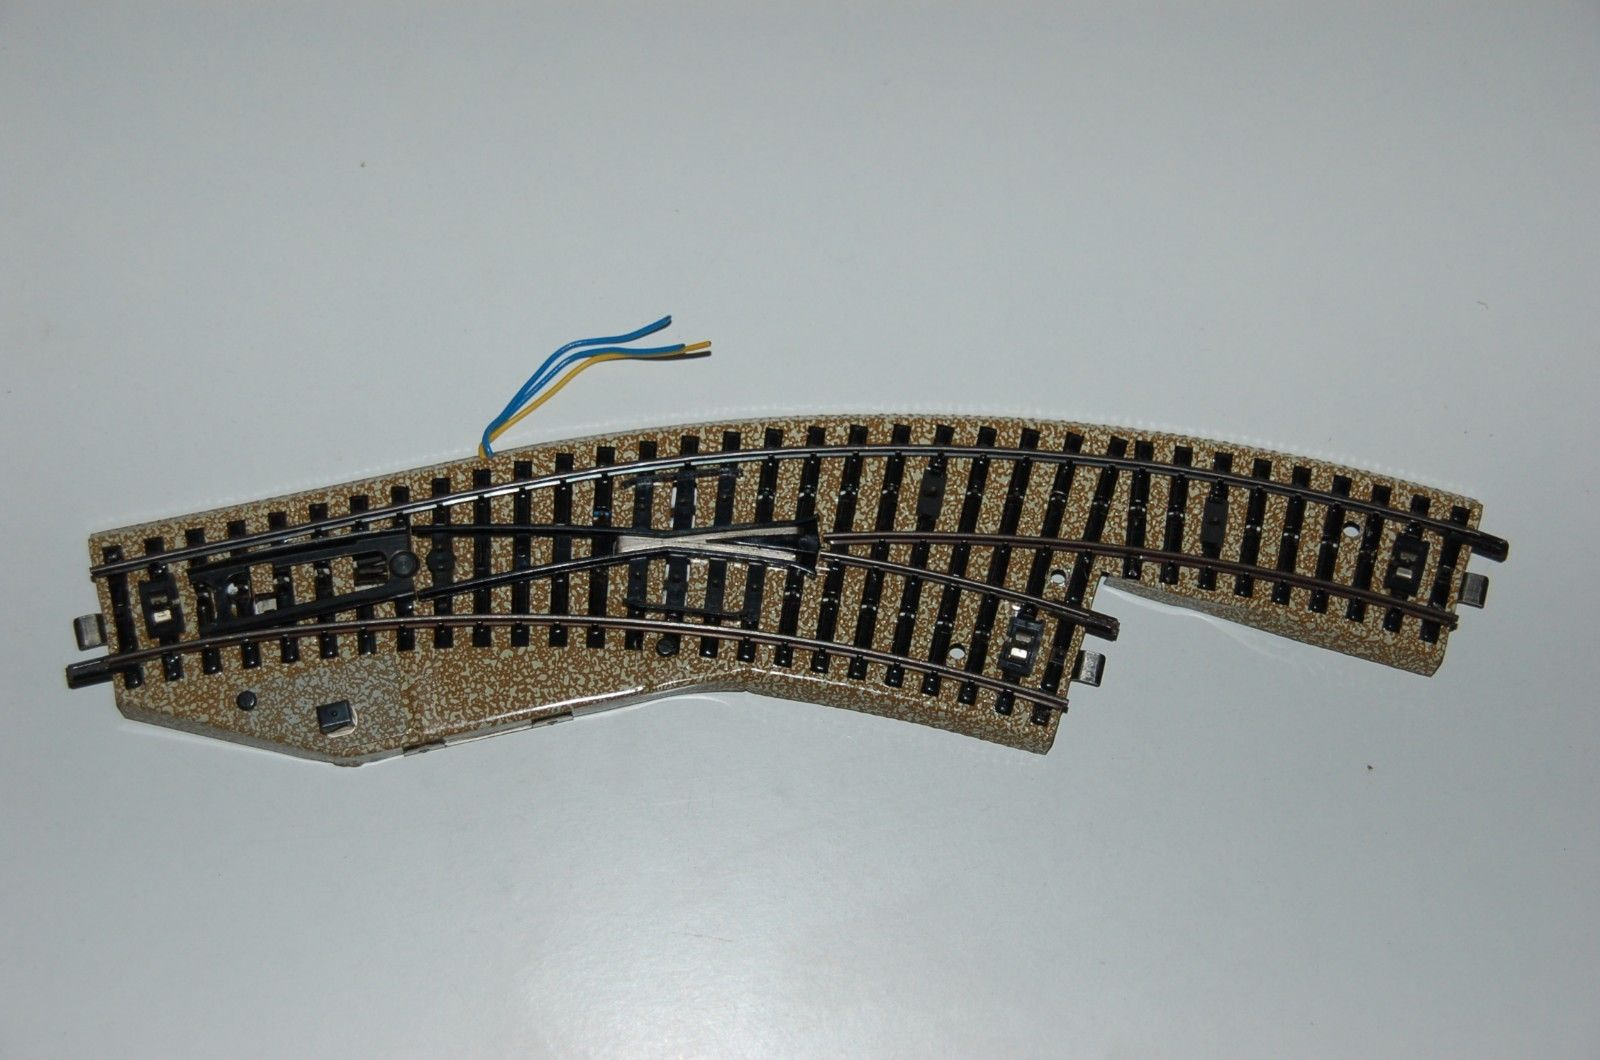
\includegraphics[width=0.2\linewidth]{img/mm5142.jpg} & 5142 (right)\\
\end{tabular}
   \caption{Curved Switch right number 5142}\label{f:5142}
\end{figure}


\begin{figure}
  \begin{center}
  {\input{SwitchNames1}}
  \end{center}
  \caption{Switches 5203 (switch left, shown on the left)
              and 5204 (switch right, shown on the right)}\label{f:switch1}
\end{figure}

Generally, tracks are continued in straight direction if the switch has a straight part.
For curced switches, the outer curve is continued.
If a switch is connected in one of the opposite directions, the connection is at the 
origin (the point, where the switch is divided into two tracks).


Regular straight switches are illustraed in in \figurename~\ref{f:switch1} where the
same three tracks are layed (stright, swithc, straight).
Naming conventions are similar for switches 5203 and 5117 as well as for switches 5204 and 5118.


\begin{figure}
  \begin{center}
  \input{SwitchNames2}
  \end{center}
  \caption{Double switches 5214 and three way turnovers}\label{f:switch2}
\end{figure}

Double switches (crossings) and three-way turnovers are shown in \figurename~\ref{f:switch2}. 
For crossings, only two connection points are allowed: O and C, as 
the other two connections would just give symmetric solutions.

%%%%%%%%%%%%%%%%%%%%%%%%%%%%%%%%%%%%%%%%%%%%%%%%%%%%%%%%%%%%%%%%%%%%%%%%%%%%%%%%%%%%%%%%%%%

\begin{verbwrite}{SwitchExample1}
\begin{tikzpicture}[scale=0.06]
  \draw (0,0) -- (100,0) -- (100,105) -- (0,105) -- cycle; %% frame

  \def\Angle{90}
  % outer
  \draw (5,55) coordinate (Start)    % start layouting tracks here
    \Rep{1}{\RCurve{5100}}
    \Rep{1}{\RCSwitch[S1][O]{5142}}
    \Rep{1}{\RCurve{5200}}
    \Rep{1}{\RCurve{5200}}
    \Rep{1}{\LCSwitch[S2][S]{5141}}
    \Rep{1}{\RCurve{5100}}
    % \Rep{2}{\RCurve{5200}}
    \Rep{3}{\RCurve{5200}}
    \Rep{3}{\RCurve{5200}}
      ;

  % inner
  \def\Angle{90} % start horizontally
  \draw ($(Start) + (7.74,0)$) % relative to Start, we lay a second loop
    \Rep{2}{\RCurve{5100}}
    \Rep{1}{\LCSwitch[S3][C]{5141}}
    \Rep{1}{\RCSwitch[S4][O]{5142}}
    \RestPosAngle{S4C}
    \Rep{3}{\RCurve{5100}}
    \Rep{3}{\RCurve{5100}}
    \Rep{3}{\RCurve{5100}}
    ;
\end{tikzpicture}
\end{verbwrite}

An example for curved switches is shown in \figurename~\ref{f:cswitch1}

\begin{figure}
  \begin{center}
  {\input{SwitchExample1}}
  \end{center}
  \caption{Example for switches}\label{f:cswitch1}
\end{figure}

%%%%%%%%%%%%%%%%%%%%%%%%%%%%%%%%%%%%%%%%%%%%%%%%%%%%%%%%%%%%%%%%%%%%%%%%%%%
\section{Up and Down}

Straight tracks can be inclined.
\begin{itemize}
  \item \texttt{Up}\{angle\} will start going uphill; the angle is given in degees,
  \item \texttt{Down}\{angle\} will start going downhill; the angle is given in degees,
  \item \texttt{Flat} will lay tracks on the current height.
\end{itemize}

%%%%%%%%%%%%%%%%%%%%%%%%%%%%%%%%%%%%%%%%%%%%%%%%%%%%%%%%%%%%%%%%%%%%%%%%%%%
\section{Bigger Examples}

A quite complex example is given in Lst.\ref{ex:example4}
The result is shown in \figurename~\ref{f:example4}.

% Reset all counters
\input{\jobname.cfg}

\begin{verbwrite}{example4}
\def\RoomLength{400}
\def\RoomWidth{250}
\begin{tikzpicture}[scale=0.040]
	\coordinate (lu) at (0,0);                     % room left
	\coordinate (lo) at (0,\RoomLength);           % room left
	\coordinate (ro) at (\RoomWidth,\RoomLength);  % room right 
	\coordinate (ru) at (\RoomWidth,0);            % room right 
	\coordinate (cu) at (120.5,\RoomLength);
	
	\draw [name path=anlage] (lu) -- (lo)  -- (ro) -- (ru) 
		-- ($(ru) - (100, 0)$) 
		-- ($(ru) - (100,-300)$) 
		-- ($(lu) - (-100,-300)$) 
		-- ($(lu) + (100,0)$) -- cycle ;

    \def\Angle{0}
    \coordinate (Start) at (56,390);
	\draw (Start)
       \Straight{5106} \Straight{5106} 
       \LSwitch[W3][S]{5203} 
       -- +(0,0) node[above] {W3}
       \Rep{5}{\Straight{5106}}
       \Rep{3}{\RCurve{5200}}
       \Straight{5109} % small correction in length
       \Rep{16}{\Straight{5106}}
       \Straight{5107}
       \Rep{6}{\RCurve{5200}}
       \Rep{4}{\Straight{5106}}
       \RCurve{5200} 
       \Rep{5}{\Straight{5106}}
       \LCurve{5100} 
       \Straight{5106} \Straight{5106} \Straight{5106} 
       \LCurve{5100} \LCurve{5100} \LCurve{5100} 
       \Straight{5106} \Straight{5107} \Straight{5106} 
       \LCurve{5100} \LCurve{5100} \LCurve{5100} 
       \Rep{12}{\Straight{5106}}
       \Straight{5107} \Straight{5106} 
       \RCurve{5200} \RCurve{5200} \RCurve{5200} \RCurve{5200} 
       \RCurve{5200} \RCurve{5200}
       \Rep{16}{\Straight{5106}}
       \Straight{5107} \Straight{5110} % small correction
       \RCurve{5200} \RCurve{5200} \RCurve{5200} \Straight{5108}
			 % -- cycle
  ;

  \def\Angle{00}
	\draw ($(Start) - (0,7.74)$)
       \Straight{5106} \LSwitch[W1][O]{5203}
       \Straight{5106} \Straight{5106} \Straight{5106} \Straight{5106} 
       \Straight{5106} \Straight{5106} \RCurve{5100} \RCurve{5100} 
       \RCurve{5100} \Straight{5109} % correction
       \Rep{16}{\Straight{5106}}
       \Straight{5107} \RCurve{5100} \RCurve{5100} \RCurve{5100} 
       \RCurve{5100} \RCurve{5100} \RCurve{5100} 
       \Rep{4}{\Straight{5106}}
       \RCurve{5100} \Straight{5106} 
       \Straight{5106} \Straight{5106} \Straight{5106} \Straight{5106}
       \LCurve{5200} \Straight{5106} \Straight{5106} \Straight{5106} 
       \LCurve{5200} \LCurve{5200} \LCurve{5200} \Straight{5106} 
       \Straight{5106} \Straight{5107} \LCurve{5200} \LCurve{5200}
       \LCurve{5200} 
       % \Straight{5106} 
       \RSwitch[W5][O]{5118}
       -- +(0,0) node[below]{W5}
       \Rep{12}{\Straight{5106}}
       \Straight{5107} \Rep{6}{\RCurve{5100}}
       \Straight{5106} \Straight{5107}
       \RSwitch[W2][O]{5118}
       -- +(0,0) node[below]{W2}
       \Rep{12}{\Straight{5106}}
       \Straight{5106} \Straight{5106} 
       \Straight{5110} % Korrektur 1
       \RCurve{5100} \RCurve{5100} \RCurve{5100} \Straight{5108}
			 % -- cycle
	;

   \RestPosAngle{W2C}
   \draw (W2C)
        \Straight{5106} 
        \Straight{5106} 
        \LSwitch[W4][O]{5203} 
       -- +(0,0) node[below]{W4}
       ;

   \RestPosAngle{W4C}
   \draw (W4C)
        \Straight{5106} 
        \Straight{5106} 
        \LCurve{5205}
        \Rep{3}{\Straight{5106}}
        \Straight{5106} 
        \Straight{5106} 
        ;

   \RestPosAngle{W4S}
   \draw (W4S)
        \Straight{5106} 
        \Straight{5106} 
        \Straight{5107} 
        \Straight{5109} 
        \Straight{5109} 
        \LCurve{5100} 
        \Straight{5106} 
        \Straight{5106} 
        \Straight{5108} 
        \Rep{4}{\Straight{5109}}
        ;

   \RestPosAngle{W5C}
   \draw (W5C)
        \LCurve{5100} 
        ;
\end{tikzpicture}
\end{verbwrite}

\Example{example4}{1}{241}{Complex example}

The tracks are shown in orthogonal projection.
This means, that tracks that are not flat will be shortened depending
on the inclination angle.

\begin{figure}
  \begin{center}
  {\input{example4}}
  \end{center}
  \caption{Example 4}\label{f:example4}
\end{figure}

There is also a macro that tells you the tracks that are used in a layout.
% This is also used in Lst~\ref{ex:example4} and the table is shown 
% \figurename~\ref{tab:example4}.
For the layout in \figurename~\ref{f:example4} this results in a table that is shown 
in \tablename~\ref{t:example4}.
% 
\begin{table}
   \centerline{\TrackUse}
   \caption{Tracks used in \figurename~\ref{f:example4}}
   \label{t:example4}
\end{table}
% \begin{figure}
% \centerline{\IfFileExists{example4.pdf}{\includegraphics[page=2,width=0.7\linewidth]{example4.pdf}}{file missing}}
%  \caption{Tracks used in Example 4}\label{tab:example4}
% \end{figure}
\section{Known Problems}

\begin{itemize}
  \item Error handling is poor.
  \item Switches have mandatory arguments with syntax for optional arguments.
     The reason is, that these arguments will become optional eventually.
  \item More documentation required.
  \item Up to now, inclination is computed only for straight tracks. How should we handle
      curves?
  \item Track types missing for Märklin (X-switch, 3 way turnover, ...)
  \item Support for other manufactureres missing (Fleischmann, Arno, ...)
  \item Configuration section currently writes definition to auxiliary file, as I did not get
      the \TeX\ expansion of the macros right -- should be solved more elegantly
  % \item Table of track pieces (e.g. \tablename~\ref{t:example4} should be multilingual
  % done
  \item Table of track pieces needs to depend on track type list in configuration section
  \item Style should have options (see comments in .sty file)
\end{itemize}
\end{document}

